\newpage
\section{Jan Jędra}
\label{sec:jjedra}

\subsection{Random mathematical equations in a list}
\begin{itemize}
\centering
    \item \[(a+b)^2=a^2+2ab+b^2\]
    \item $ r=\frac{C}{2\pi}$
\end{itemize}

\subsection{Photo of a gorilla}

\begin{flushleft}
\textbf{Gorillas} (see Figure~\ref{fig:gorilla}) are herbivorous, predominantly ground-dwelling great apes that inhabit the tropical forests of equatorial Africa. The genus Gorilla is divided into two species: the eastern gorilla and the western gorilla, and either four or five subspecies. The DNA of gorillas is highly similar to that of humans, from \underline{95 to 99\%} depending on what is included, and they are the next closest living relatives to humans after chimpanzees and bonobos.\par
\textbf{Gorillas} are the \textbf{largest} living primates, reaching heights between 1.25 and 1.8 metres, weights between 100 and 270 kg, and arm spans up to 2.6 metres, depending on species and sex. They tend to live in troops, with the leader being called a \textit{silverback}. The Eastern gorilla is distinguished from the Western by darker fur colour and some other minor morphological differences. Gorillas tend to live 35–40 years in the wild.
\end{flushleft}
\begin{figure}[htbp]
    \centering
    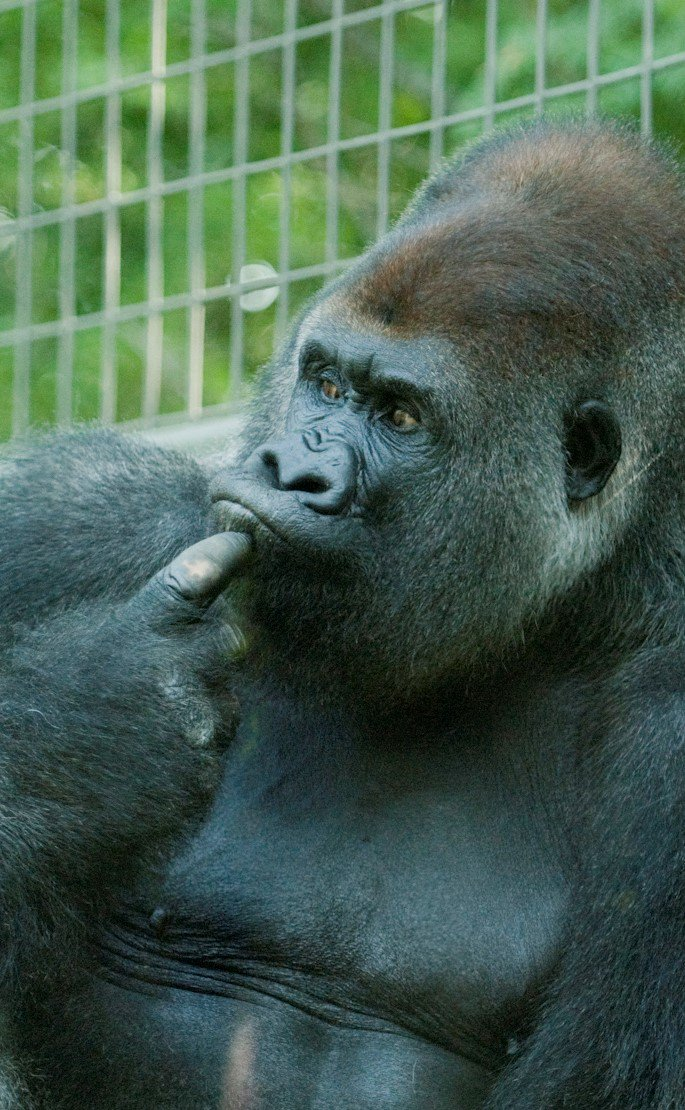
\includegraphics[width=0.4\textwidth]{pictures/gorilla.jpg}
    \caption{His name is Olivier}
    \label{fig:gorilla}
\end{figure}

\newpage
Table~\ref{tab:multiplication_table} represents multiplication of numbers between 1 and 4.
\begin{table}[htbp]
\centering
\begin{tabular}{lllll}
                       & 1                      & 2                      & 3                       & 4                       \\ \cline{2-5} 
\multicolumn{1}{l|}{1} & \multicolumn{1}{l|}{1} & \multicolumn{1}{l|}{2} & \multicolumn{1}{l|}{3}  & \multicolumn{1}{l|}{4}  \\ \cline{2-5} 
\multicolumn{1}{l|}{2} & \multicolumn{1}{l|}{2} & \multicolumn{1}{l|}{4} & \multicolumn{1}{l|}{6}  & \multicolumn{1}{l|}{8}  \\ \cline{2-5} 
\multicolumn{1}{l|}{3} & \multicolumn{1}{l|}{3} & \multicolumn{1}{l|}{6} & \multicolumn{1}{l|}{9}  & \multicolumn{1}{l|}{12} \\ \cline{2-5} 
\multicolumn{1}{l|}{4} & \multicolumn{1}{l|}{4} & \multicolumn{1}{l|}{8} & \multicolumn{1}{l|}{12} & \multicolumn{1}{l|}{16} \\ \cline{2-5} 
\end{tabular}
\label{tab:multiplication_table}
\caption{Multiplication table}
\end{table}
\hline
\subsection{\hspace{2em}Gorilla names.}
Examples of gorilla names:
\begin{enumerate}
    \item Olivier
    \item Winston
    \item Koko
\end{enumerate}